
\section{Viabilidade econômica}
A viabilidade econômica do projeto possui fatores limitantes como o orçamento pré-definido de R\$4000,00 (quatro mil reais), custos dos materiais que compõem o projeto, custo dos componentes para montagem do protótipo, e uma série de custos pós-venda do produto. \\

Sendo um projeto de relevante complexidade e especificidade, o público alvo para venda é bastante restrito, trazendo pontos positivos e negativos ao desenvolvimento de um plano de vendas. Dentre os pontos positivos, pode ser citada a possível fidelização do cliente com os desenvolvedores do sistema de arrefecimento para o sensor, visto que poucas empresas são voltadas exclusivamente aos projetos de cunho universitário que abordam esse tema. Além disso, uma menor quantia será gasta com prospecção ativa, visto que a própria apresentação do serviço do cliente para outro público já aumenta consideravelmente o interesse da comunidade acadêmica pela solução apresentada por este projeto. \\

Por outro lado, do ponto de vista negativo, nenhum dos componentes materiais do sistema são fabricados pelos idealizadores do projeto. Além disso, o próprio código feito para o Arduino é de domínio público, obrigando assim a disponibilização do código fonte para qualquer concorrente que requeira este arquivo. Dessa forma, caso os programadores destas empresas criassem um sistema melhor, e alterassem o código ao seu favor, o projeto desenvolvido pelo grupo se tornaria ultrapassado no mercado.\\ 

A análise de viabilidade deste projeto não levou em consideração o custo das horas trabalhadas por estudante, visto que com um grupo de 30 estudantes, o projeto já começaria inválido, pois o preço médio de um estágio de engenharia é de aproximadamente 1000 reais por 120 horas mensais, o que resultaria em R\$30.000 de mão-de-obra. Além disso, esses dados são referentes apenas a um mês de trabalho, sendo que o projeto em questão teve duração de um semestre para desenvolvimento. \\

Partindo para a análise dos custos com materiais, os valores referentes a protótipos, softwares de dimensionamento, e ferramentas para simulações, geraram os gastos especificados na tabela ~\ref{tab1ve} a seguir 
\begin{table}[!htb]
	\centering
	\caption{Preços do protótipo}\label{tab1ve}
	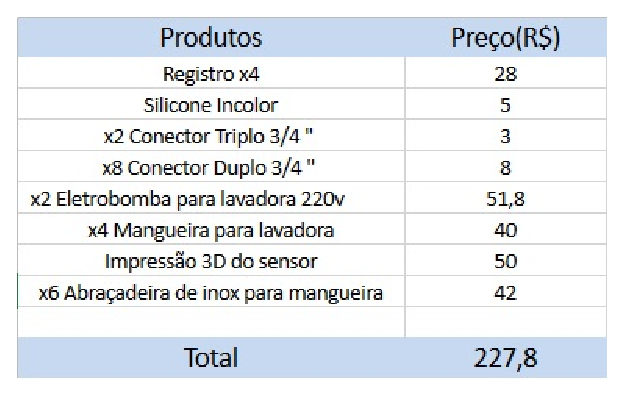
\includegraphics[scale=1]{figuras/figura1ve.eps}
\end{table} 
\newpage
O custeamento total está descrito nas tabelas ~\ref{tab2ve} e ~\ref{tab3ve} abaixo. Caso o cliente já possua a placa em questão, os gastos pré-venda são reduzidos significativamente, e consequentemente o valor do custo final do projeto também é menor\\ 
\begin{table}[!htb]
	\centering
	\caption{Preço dos setores físicos}\label{tab2ve}
	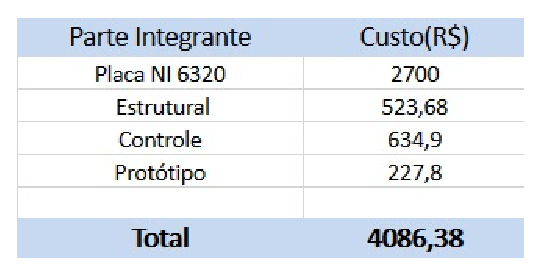
\includegraphics[scale=1]{figuras/figura2ve.eps}
\end{table}
\begin{table}[htbp]
	\centering
	\caption{Preço específico dos setores físicos }
	\begin{longtable}{rcrc|p{4.855em}|r|}
		\toprule
		\rowcolor[rgb]{ 0,  0,  0} \multicolumn{1}{|p{6.07em}|}{\textcolor[rgb]{ 1,  1,  1}{\textbf{Componente}}} & \multicolumn{1}{p{7.215em}|}{\textcolor[rgb]{ 1,  1,  1}{\textbf{Modelo}}} & \multicolumn{1}{c|}{\textcolor[rgb]{ 1,  1,  1}{\textbf{Fornecedor}}} & \textcolor[rgb]{ 1,  1,  1}{\textbf{Quantidade}} & \textcolor[rgb]{ 1,  1,  1}{\textbf{Orçamento unitário}} & \multicolumn{1}{c|}{\textcolor[rgb]{ 1,  1,  1}{\textbf{Orçamento}}} \\
		\midrule
		\endfirsthead
		\toprule
		\rowcolor[rgb]{ 0,  0,  0} \multicolumn{1}{|p{6.07em}|}{\textcolor[rgb]{ 1,  1,  1}{\textbf{Componente}}} & \multicolumn{1}{p{7.215em}|}{\textcolor[rgb]{ 1,  1,  1}{\textbf{Modelo}}} & \multicolumn{1}{c|}{\textcolor[rgb]{ 1,  1,  1}{\textbf{Fornecedor}}} & \textcolor[rgb]{ 1,  1,  1}{\textbf{Quantidade}} & \textcolor[rgb]{ 1,  1,  1}{\textbf{Orçamento unitário}} & \multicolumn{1}{c|}{\textcolor[rgb]{ 1,  1,  1}{\textbf{Orçamento}}} \\
		\midrule
		\endhead
		\hline
		\endfoot
		\hline\hline
		\endlastfoot
		\rowcolor[rgb]{ .851,  .851,  .851} \multicolumn{1}{|p{6.07em}|}{Bomba} & \multicolumn{1}{p{7.215em}|}{DC30QA-1230 } & \multicolumn{1}{l|}{Ali Express} & 2     & \multicolumn{1}{r|}{R\$ 33,48} & R\$ 66,96 \\
		\midrule
		\multicolumn{1}{|p{6.07em}|}{Radiador} & \multicolumn{1}{p{7.215em}|}{Radiador de alumínio com conexões G $1/4$, 240 mm} & \multicolumn{1}{l|}{Mercado Livre} & 1     & \multicolumn{1}{r|}{R\$ 150,00} & R\$ 150,00 \\
		\midrule
		\rowcolor[rgb]{ .851,  .851,  .851} \multicolumn{1}{|p{6.07em}|}{Cooler} & \multicolumn{1}{p{7.215em}|}{Cooler FAN “CoolerMaster Sickleflow 12cm R4-SXDP-20FB-R1} & \multicolumn{1}{l|}{Kabum} & 4     & \multicolumn{1}{r|}{R\$ 35,18} & R\$ 140,72 \\
		\midrule
		\multicolumn{1}{|p{6.07em}|}{Tubulação} & \multicolumn{1}{p{7.215em}}{Politetrafluoretileno (PTFE), } & \multicolumn{1}{l|}{HOESCHT} & 8     & \multicolumn{1}{r|}{R\$ 4,50} & R\$ 36,00 \\
		\rowcolor[rgb]{ .851,  .851,  .851} \multicolumn{1}{|p{6.07em}|}{Conectores} & \multicolumn{1}{p{7.215em}|}{Swagelok, Latão} & \multicolumn{1}{l|}{Swagelok} & 13    & \multicolumn{1}{r|}{R\$ 5,00} & R\$ 65,00 \\
		\midrule
		\multicolumn{1}{|p{6.07em}|}{Reservatório} & \multicolumn{1}{p{7.215em}|}{PEAD (Polietileno de Alta Densidade) de 15 x 33 x 22 cm} & \multicolumn{1}{p{6.43em}|}{Mercado Livre} & 1     & \multicolumn{1}{r|}{R\$ 40,00} & R\$ 40,00 \\
		\midrule
		\rowcolor[rgb]{ .851,  .851,  .851} \multicolumn{1}{|p{6.07em}|}{Válvulas} & \multicolumn{1}{p{7.215em}|}{VALVULA DUPLA DE ENTRADA DE AGUA LAVADORA ELECTROLUX } & \multicolumn{1}{p{6.43em}|}{Mercado Livre} & 2     & \multicolumn{1}{r|}{R\$ 45,00} & R\$ 90,00 \\
		\midrule
		\multicolumn{1}{|p{6.07em}|}{Sensor de Temperatura - Adaptador } & \multicolumn{1}{p{7.215em}|}{TJ36-CASS-116G-6-CC-XCIB} & \multicolumn{1}{l|}{Omega} & 1     & \multicolumn{1}{r|}{R\$ 382,00} & R\$ 382,00 \\
		\midrule		
		\rowcolor[rgb]{ .851,  .851,  .851} \multicolumn{1}{|p{6.07em}|}{Sensor de Temperatura - Tubulação} & \multicolumn{1}{p{7.215em}|}{Sensor de Temperatura DS18B20} & \multicolumn{1}{l|}{Usinainfo} & 1     & \multicolumn{1}{r|}{R\$ 16,80} & R\$ 16,80 \\
		\midrule
		\multicolumn{1}{|p{6.07em}|}{Sensor de Temperatura - Reservatório} & \multicolumn{1}{p{7.215em}|}{Sensor de Temperatura DS18B20} & \multicolumn{1}{l|}{Usinainfo} & 1     & \multicolumn{1}{r|}{R\$ 16,80} & R\$ 16,80 \\
		\midrule
		\rowcolor[rgb]{ .851,  .851,  .851} \multicolumn{1}{|p{6.07em}|}{Sensor de Fluxo - Tubulação} & \multicolumn{1}{p{7.215em}}{YF-S401} & \multicolumn{1}{l|}{Mercado Livre} & 1     & \multicolumn{1}{r|}{R\$ 28,80} & R\$ 28,80 \\
		\multicolumn{1}{|p{6.07em}|}{Sensor de Pressão - Tubulação} & \multicolumn{1}{p{7.215em}|}{MPX 2200 GP} & \multicolumn{1}{l|}{Mercado Livre} & 1     & \multicolumn{1}{r|}{R\$ 55,00} & R\$ 55,00 \\
		\midrule
		\rowcolor[rgb]{ .851,  .851,  .851} \multicolumn{1}{|p{6.07em}|}{Sensor de Nível - Reservatório} & \multicolumn{1}{p{7.215em}|}{Não Especificado} & \multicolumn{1}{p{6.43em}|}{Usinainfo} & 1     & \multicolumn{1}{r|}{R\$ 24,90} & R\$ 24,90 \\
		\midrule
	\end{longtable}
	\label{tab3ve}
\end{table}
	\newpage
	\begin{table}[htbp]
		\centering
		\begin{tabular}{rcrc|p{4.855em}|r|}
			\toprule
			\rowcolor[rgb]{ 0,  0,  0} \multicolumn{1}{|p{6.07em}|}{\textcolor[rgb]{ 1,  1,  1}{\textbf{Componente}}} & \multicolumn{1}{p{7.215em}|}{\textcolor[rgb]{ 1,  1,  1}{\textbf{Modelo}}} & \multicolumn{1}{c|}{\textcolor[rgb]{ 1,  1,  1}{\textbf{Fornecedor}}} & \textcolor[rgb]{ 1,  1,  1}{\textbf{Quantidade}} & \textcolor[rgb]{ 1,  1,  1}{\textbf{Orçamento unitário}} & \multicolumn{1}{c|}{\textcolor[rgb]{ 1,  1,  1}{\textbf{Orçamento}}} \\
			\midrule
			\multicolumn{1}{|p{6.07em}|}{Placa de Processamento} & \multicolumn{1}{p{7.215em}|}{Arduino Uno Rev3} & \multicolumn{1}{p{6.43em}|}{Filipeflop} & 1     & \multicolumn{1}{r|}{R\$ 47,90} & R\$ 47,90 \\
			\rowcolor[rgb]{ .851,  .851,  .851} \multicolumn{1}{|p{6.07em}|}{Módulo Relé 5V 10A 2 Canais} & \multicolumn{1}{p{7.215em}|}{SRD-05VDC-SL-C} & \multicolumn{1}{l|}{Filipeflop} & 1     & \multicolumn{1}{r|}{R\$ 12,90} & R\$ 12,90 \\
			\midrule
			\multicolumn{1}{|p{6.07em}|}{Módulo Relé 5V 10A 4 Canais} & \multicolumn{1}{p{7.215em}|}{SRD-05VDC-SL-C} & \multicolumn{1}{l|}{Filipeflop} & 2     & \multicolumn{1}{r|}{R\$ 24,90} & R\$ 49,80 \\
			\midrule
			&       &       &       & Subtotal: & R\$ 1.223,58 \\
			\cmidrule{5-6}    \end{tabular}%
		\label{tab:addlabel}%
	\end{table}%
	
Os custos pós-venda, tais como: manutenção do sistema, instalação do sistema no local para testes, e transporte do produto até o local, dependem de uma série de fatores que são difíceis de mensurar quantitativamente. Por exemplo: caso o erro seja em apenas um sensor, o custo para manutenção dependeria da situação a qual o sensor se encontra (deve-se comprar um novo? ele é recuperável?), da distância cujos integrantes percorreriam para fazer a manutenção (quantos seriam necessários para arrumar o problema? eles teriam acomodação, caso fosse um local distante?). Esse tipo de análise foge do escopo deste relatório, apesar de ser um fator de extrema importância na decisão da viabilidade econômica do produto. 

Com todos esses pontos estudados, é possível definir, de modo pouco acurado que, para um orçamento inicial estipulado de R\$4000,00 (quatro mil reais) apenas para o sistema de arrefecimento, o projeto é viável economicamente. 

	
	
	
	
